% ###########################################################
%
% LaTeX Template for undergraduate thesis book and report
%
% Author: Md. Ashiqur Rahman (Opu)
% Roll: 1007035
% 
% Special Contents:
%   * Sub-figures
%   * Tikz Image for flowchart
%
% Rename the chapters as per your requirements
%
% Please do not remove Template author name from this file
%
% ###########################################################


\documentclass[12pt]{report}
\usepackage[utf8x]{inputenc}
\usepackage{graphicx}
\graphicspath{{images/}}
\usepackage{hyperref}
%\usepackage{chngpage}
%\usepackage{subfig}
%\usepackage{subfigure}
%\usepackage{float}
\usepackage[a4paper,tmargin=1.1in,bmargin=1.1in,lmargin=1.2in,rmargin=1in]{geometry}
%\usepackage{fancyhdr}
%\pagestyle{fancy}
\usepackage{enumitem}
\usepackage[algoruled,boxed,lined]{algorithm2e}
\usepackage{graphicx}
\usepackage{caption}
\usepackage[font={scriptsize}]{subcaption}
%\usepackage{subcaption}
\usepackage{array}
\usepackage{tikz}
\usetikzlibrary{shapes.geometric,arrows,positioning}
\tikzstyle{startstop}=[ellipse, minimum width=3cm, minimum height=0.6cm,text centered, draw=black, fill=white]
\tikzstyle{io}=[trapezium, trapezium left angle=70, trapezium right angle=110, minimum width=3cm, minimum height=0.6cm, text centered, draw=black, fill=white]
\tikzstyle{process}=[rectangle, minimum width=2cm, minimum height=0.6cm, text centered, draw=black, fill=white]
\tikzstyle{decision}=[diamond, aspect=2, minimum width=1.5cm, minimum height=0.8cm, text centered, draw=black, fill=white]
\tikzstyle{arrow} = [thick,->,>=stealth]
\tikzset{draw}

\usepackage{amsthm}
\usepackage{amsmath}
\usepackage{amssymb}

\theoremstyle{plain}
\newtheorem{thm}{Theorem}[chapter] % reset theorem numbering for each chapter
\newtheorem{theory}{Theorem}
\newtheorem{tlem}{Theorem}
\newtheorem{texmpl}{Theorem}
\theoremstyle{definition}
\newtheorem{defn}[thm]{Definition} % definition numbers are dependent on theorem numbers
\newtheorem{exmp}[texmpl]{Example} % same for example numbers
\newtheorem{lem}[tlem]{Lemma}

\newcommand\textbox[1]{%
  \parbox{.333\textwidth}{#1}%
}


\usepackage{titlesec}
 

\makeatletter
\def\@makechapterhead#1{%
  \vspace*{0\p@}%
  {\parindent \z@ \centering
    \normalfont
    \ifnum \c@secnumdepth >\m@ne
      \if@mainmatter
        \large \bfseries \@chapapp\space \thechapter
        \par\nobreak
        \vskip 20\p@
      \fi
    \fi
    \interlinepenalty\@M
    \LARGE \bfseries #1\par\nobreak
    \vskip 40\p@
  }}
\def\@schapter#1{\if@twocolumn
                   \@topnewpage[\@makeschapterhead{#1}]%
                 \else
                   \@makeschapterhead{#1}%
                   \@afterheading
                 \fi}
\def\@makeschapterhead#1{%
  \vspace*{0\p@}%
  {\parindent \z@ \centering
    \normalfont
    \interlinepenalty\@M
    \Large \bfseries  #1\par\nobreak
    \vskip 40\p@
  }}

\renewcommand\section{\@startsection {section}{1}{\z@}%
                                   {-6ex \@plus -1ex \@minus -.2ex}%
                                   {2.3ex \@plus.2ex}%
                                   {\normalfont\Large\bfseries}}

\renewcommand\subsection{\@startsection {subsection}{1}{\z@}%
                                   {-4ex \@plus -1ex \@minus -.2ex}%
                                   {2.3ex \@plus.2ex}%
                                   {\normalfont\large\bfseries}}

\makeatother

\begin{document}

\pagenumbering{roman}
\setcounter{page}{1}


% ############################################################################################################
%
% Title Page (only if you want to make it with LaTeX)
%
\begin{figure}
  \centering
  
\includegraphics[width=2cm]{kuetlogo.png}
\end{figure}

\title{
    {An Approach for Multi Label Image Classification Using Single Label Convolutional Neural Network Classifier with Objectness Measure and Selective Search}\\
    {
\includegraphics[width=4cm]{gap.png}}\\
    {
\includegraphics[width=4cm]{gap.png}}\\
    {
\includegraphics[width=4cm]{gap.png}}\\
}

\author{Setu Basak\\
        Roll: 1107043\\
        Shubhashis Karmakar\\
        Roll: 1107001\\\\
        Supervisor: Dr. Kazi Md. Rokibul Alam\\
        Professor, CSE, KUET\\\\\\
}

\date{April, 2016}
%
% ############################################################################################################



\setlength{\parindent}{1em}
%\setlength{\parskip}{1em}

%\usepackage{titlesec}

\titlespacing*{\section}
{0pt}{5.5ex plus 1ex minus .2ex}{4.3ex plus .2ex}
\titlespacing*{\subsection}
{0pt}{5.5ex plus 1ex minus .2ex}{4.3ex plus .2ex}

%\begin{document}

\maketitle

\addtocontents{toc}{~\hfill\textbf{Page}\par}

\chapter*{Acknowledgement}
\addcontentsline{toc}{chapter}{Acknowledgement}
%\renewcommand{\abstractname}{Acknowledgements}
%\begin{abstract}
With due homage and honor, we want to express our gratitude to Almighty Allah.\\


\noindent We express our indebtedness to our dedicated supervisor Dr. Kazi Md. Rokibul Alam (Professor, Department of Computer Science and Engineering, KUET) for his necessary guidance, suggestions and encouragement to all phases of our work. We
would also like to thank all the teachers who've been much helpful and encouraging in completion of our thesis work.\\

\noindent\textbox{\hfill}\textbox{\hfil \hfil}\textbox{\hfill \textbf{Authors}}
%\end{abstract}

\chapter*{Abstract}
\addcontentsline{toc}{chapter}{Abstract}
%\renewcommand{\abstractname}{Abstract}
%\begin{abstract}
Single label image classification has been promisingly demonstrated using Convolutional Neural Network (CNN). However, how this CNN will fit for multi-label images is still difficult to solve. It is mainly difficult due to the complex underlying
object layouts and insufficient multi-label training images. In this work, we propose an approach for classifying multi-label image by a trained single label classifier using CNN with objectness measure and selective search. We took two established image segmentation techniques for segmenting a single image which is a multi-label image into some segmented images. Then we forwarded the images to our trained CNN and predicted the labels of the segmented images by generalizing the result. Our single-label image classifier gives 87\% accuracy on CIFAR-10 dataset. Using objectness measure with CNN gives us 51\% accuracy on a multi-label dataset and gives upto 57\% accuracy using selective search both considering top-4 labels which is significantly good for a simple approach rather than a complex approach of multi-label classifier using CNN.

%\end{abstract}


%\chapter*{Dedication}
%To mum and dad

\tableofcontents
%\addcontentsline{toc}{chapter}{Contents}
\listoffigures
\addcontentsline{toc}{chapter}{List of Figures}
%\listoftables
%\addcontentsline{toc}{chapter}{List of Tables}

%\setlength{\parskip}{1ex plus 0.5ex minus 0.2ex}

\chapter{Introduction}
\setcounter{page}{2}
\pagenumbering{arabic}
\section{Background}
Image classification containing a single-label, which
has been extensively studied in the recent
years \cite{1}, \cite{2}. For image representation and
classification, conventional approaches utilize carefully designed hand-crafted features, e.g., SIFT \cite{3},
along with the bag-of-words coding scheme, followed
by the feature pooling \cite{4}, \cite{5} and classic
classifiers, such as Support Vector Machine (SVM) \cite{6}
and random forests \cite{7}. Recently, in contrast to the
hand-crafted features, learnt image features with deep
network structures  have shown their great potential
in various vision recognition tasks \cite{8}, \cite{9}, \cite{10},
\cite{11}. Among these architectures, one of the greatest breakthroughs in image classification is the deep
convolutional neural network (CNN) \cite{10}, which has
achieved the state-of-the-art performance (with 10\%
gain over the previous methods based on handcrafted features) in the large-scale single-label object
recognition task, i.e., ImageNet Large Scale Visual
Recognition Challenge (ILSVRC) \cite{2} with more than
one million images from 1,000 object categories.\hfill \break

Multi-label image classification is however a more
general and practical problem, since the majority of real-world images are with more than one objects
of different categories. Many methods \cite{12}, \cite{13}, \cite{14}
have been proposed to address this more challenging
problem. The success of CNN on single-label image
classification also sheds some light on the multi-label image classification problem. However, the CNN
model cannot be trivially extended to cope with the
multi-label image classification problem in an interpretable manner, mainly due to the following reasons.
Firstly, the implicit assumption that foreground objects are roughly aligned, which is usually true for
single-label images, does not always hold for multi-label images. Such alignment facilitates the design of
the convolution and pooling infrastructure of CNN
for single-label image classification. However, for a
typical multi-label image, different categories of objects are located at various positions with different
scales and poses. For example, as shown in Figure \ref{fig1},
for single-label images, the foreground objects are
roughly aligned, while for multi-label images, even
with the same label, i.e., cat and bird, the spatial arrangements of the cat and bird instances
vary largely among different images. Secondly, the
interaction between different objects in multi-label
images, like partial visibility and occlusion, also poses
a great challenge. Therefore, directly applying the
original CNN structure for multi-label image classification is not feasible. Thirdly, due to the tremendous
parameters to be learned for CNN, a large number of
training images are required for the model training.
Furthermore, from single-label to multi-label (with n
category labels) image classification, the label space
has been expanded from n to 2n, thus more training data is required to cover the whole label space. For
single-label images, it is practically easy to collect
and annotate the images. However, the burden of
collection and annotation for a large scale multi-label
image dataset is generally extremely high. \hfill \break

So we propose a simple technique using our trained single-label classifier of CNN with the objectness measure \cite{15} and selective search \cite{16}. First we segment a multi-label image into some segments or image windows using the two approaches and then test these images against our trained single label model and predict the multiple labels of the image. We have taken different approaches like taking top-1, top-2, total sum of the scores and cumulative percentage sum of the scores to predict the labels.

\begin{figure}[ht] 
  \begin{subfigure}[b]{0.25\linewidth}
    \centering
    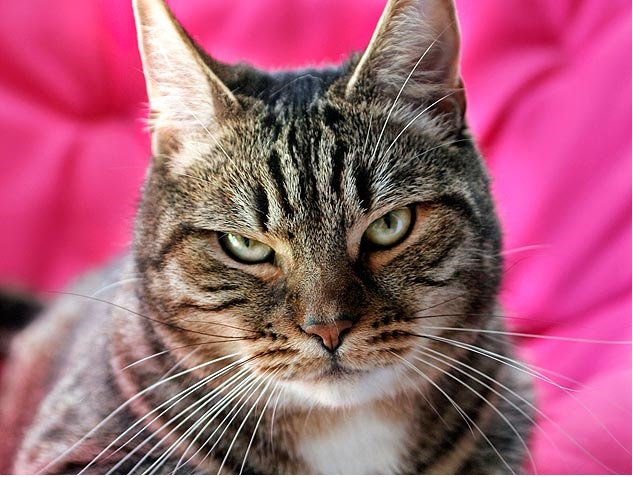
\includegraphics[width=0.5\linewidth]{1a}
    \caption{} 
    \label{1a} 
    \vspace{4ex}
  \end{subfigure}%%
  \begin{subfigure}[b]{0.25\linewidth}
    \centering
    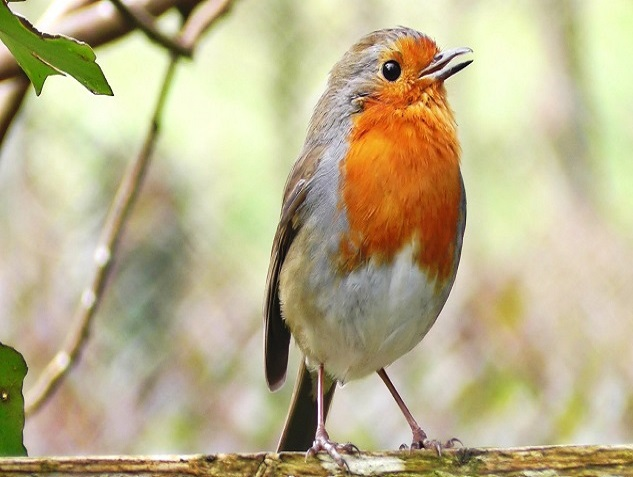
\includegraphics[width=0.5\linewidth]{1b}
    \caption{} 
    \label{1b} 
    \vspace{4ex}
  \end{subfigure}%%
  \begin{subfigure}[b]{0.25\linewidth}
    \centering
    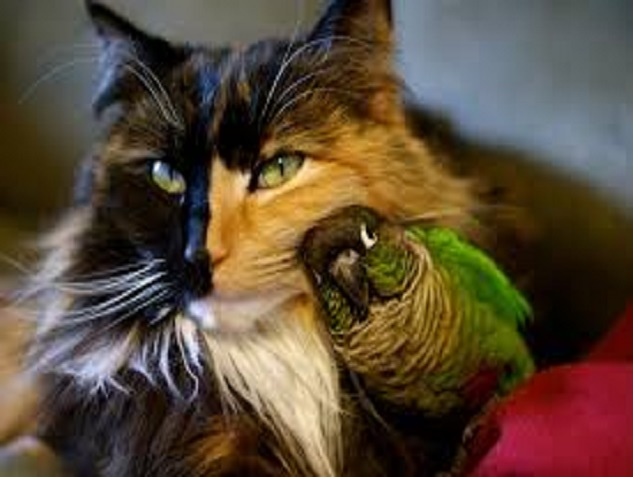
\includegraphics[width=0.5\linewidth]{1c} 
    \caption{} 
    \label{1c} 
    \vspace{4ex}
  \end{subfigure}%%
  \begin{subfigure}[b]{0.25\linewidth}
    \centering
    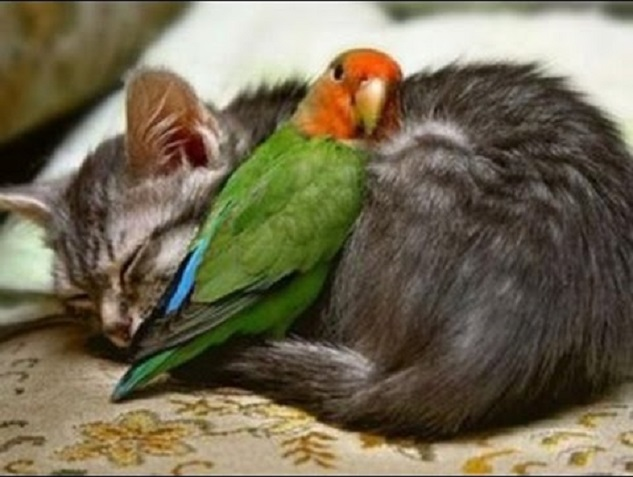
\includegraphics[width=0.5\linewidth]{1d} 
    \caption{} 
    \label{1d}
    \vspace{4ex} 
    \end{subfigure}
  \caption{(a),(b)Some examples from CIFAR-10 \cite{17}. The objects in single-label
images are usually roughly aligned.(c),(d) However, the assumption of object alignment is not valid for multi-label
images. Also note the partial visibility and occlusion
between objects in the multi-label images.}
  \label{fig1} 
\end{figure}

\section{Motivation}
The major, recurrent theme throughout this work is our search for a good generative model for labeling of natural
images. In addition, we seek a model with image segmentation based on objectness measure and selective search that is capable of extracting multiple labels from images. The hope is that we would find out a simple model that can classify multiple labels. Finally, the training time for the model would be small and segmenting the images would be easy enough.

\section{Problem Statement}\label{sec:ProbStatement}
Being able to automatically detect the multiple labels of an
image is a very
challenging task, but it could have great impact, for instance
by helping visually impaired people better identify the
content of images on the web. This task is significantly
harder, for example, than the well-studied image classification or object recognition tasks, which have been a main
focus in the computer vision community. It is also very tough to get dataset of multiple images and train it for a model. That model will be huge and will take loads of time. So our task will be as follows:

% List items using numbering
\begin{enumerate}
  \item To predict a single label image.
  \item Segmentation of an image containing multiple objects into some segmented images using objectness measure \cite{15} and selective search \cite{16}.
  \item Using the segmented images to predict multiple labels in an image. 
\end{enumerate}


\section{Objectives}
% List items using bullets

\begin{itemize}
  \item First objective is to maximize the accuracy of single-label image detection using Convolutional Neural Network(CNN).
  \item Next objective is to produce image windows from an image having multiple objects using objectness measure and selective search.
  \item Last objective is to predict labels of an image using top-1, top-2, total score sum and cumulative percentage sum of the score of every segmented images.
\end{itemize}




\chapter{Related Works}
During the past few years, many works on various
multi-label image classification models have been conducted. These models are generally based on two
types of frameworks: bag-of-words (BoW) \cite{18}, \cite{12},
\cite{13}, \cite{14} and deep learning \cite{19}.

\section{Bag-of-Words Based Models}

A traditional BoW model is composed of multiple
modules, e.g., feature representation, classification
and context modeling. For feature representation,
the main components include hand-crafted feature
extraction, feature coding and feature pooling, which
generate global representations for images. Specifically, hand-crafted features, such as SIFT \cite{3}, Histogram of Oriented Gradients \cite{20} and Local Binary
Patterns \cite{21} are firstly extracted on dense grids or
sparse interest points and then quantized by different
coding schemes, e.g., Vector Quantization \cite{22}, Sparse
Coding and Gaussian Mixture Models \cite{23}. These
encoded features are finally pooled by feature aggregation methods, such as Spatial Pyramid Matching
(SPM) \cite{4}, to form the image-level representation. For
classification, conventional models, such as SVM \cite{6}
and random forests \cite{7}, are utilized. Beyond conventional modeling methods, many recent works \cite{18}, \cite{13} have demonstrated that the usage
of context information, e.g., spatial location of object
and background scene from the global view, can
considerably improve the performance of multi-label
classification and object detection. \hfill \break

Although these works have made great progress
in visual recognition tasks, the involved hand-crafted
features are not always optimal for particular tasks.
Recently, in contrast to hand-crafted features, learnt
features with deep learning structures have shown
great potential for various vision recognition tasks,
which will be introduced in the following subsection.

\section{Deep Learning Based Models}

Deep learning tries to model the high-level abstractions of visual data by using architectures composed of multiple non-linear transformations. Specifically, deep convolutional neural network (CNN) \cite{8}
has demonstrated an extraordinary ability for image classification \cite{9}, \cite{10} on single-label datasets such as CIFAR-10/100 \cite{17} and ImageNet \cite{2}.
More recently, CNN architectures have been
adopted to address multi-label problems. Gong et
al. \cite{19} studied and compared several multi-label
loss functions for the multi-label annotation problem
based on a similar network structure to \cite{10}. However,
due to the large number of parameters to be learned
for CNN, an effective model requires lots of training
samples. Therefore, training a task-specific convolutional neural network is not applicable on datasets
with limited numbers of training samples.









\chapter{Initial Attempts}
Before migrating to Convolutional Neural Network(CNN) we tried many simple approaches for single-label image classification which we would use as a trained model for multi-label image classification. Though the accuracy of the approaches were not that good and also had many difficulties.

\section{Nearest Neighbor Classifier} 

The nearest neighbor classifier will take a test image, compare it to every single one of the training images, and predict the label of the closest training image. We compare the images pixel by pixel and add up all the differences. In other words, given two images and representing them as vectors $\big(I_{1},I_{2}\big)$ , a reasonable choice for comparing them might be the L1 distance:

\begin{equation}
 d_{1}(I_{1},I_{2}) =\sum_{p} \big(I_{1}^p-I_{2}^p\big)
\end{equation}

There are many other ways of computing distances between vectors. We can use the L2 distance, which has the geometric interpretation of computing the euclidean distance between two vectors.


\begin{equation}
 d_{1}(I_{1},I_{2}) = \sqrt{\sum_{p} \big(I_{1}^p-I_{2}^p\big)}
 \end{equation}
 
\paragraph{Accuracy}
\leavevmode \\
We got about $35\%$ using the NN Classifier.



\subsection{k - Nearest Neighbor Classifier}
Instead of finding the single closest image in the training set, we will find the top k closest images, and have them vote on the label of the test image. In particular, when k = 1, we recover the Nearest Neighbor classifier. The k-nearest neighbor classifier requires a setting for k. But what number works best? We have tried out many different values of k and experimented what k value works best.

\subsection{Cross-validation}
In cases where the size of the training data (and therefore also the validation data) is small, we can use a hyperparameter tuning called cross-validation. Instead of arbitrarily picking datapoints to be the validation set and rest training set, we can get a better and less noisy estimate of how well a certain value of k works by iterating over different validation sets and averaging the performance across these. For example, in 5-fold cross-validation, we would split the training data into 5 equal folds, use 4 of them for training, and 1 for validation.
\begin{figure}[h!]
  \centering
  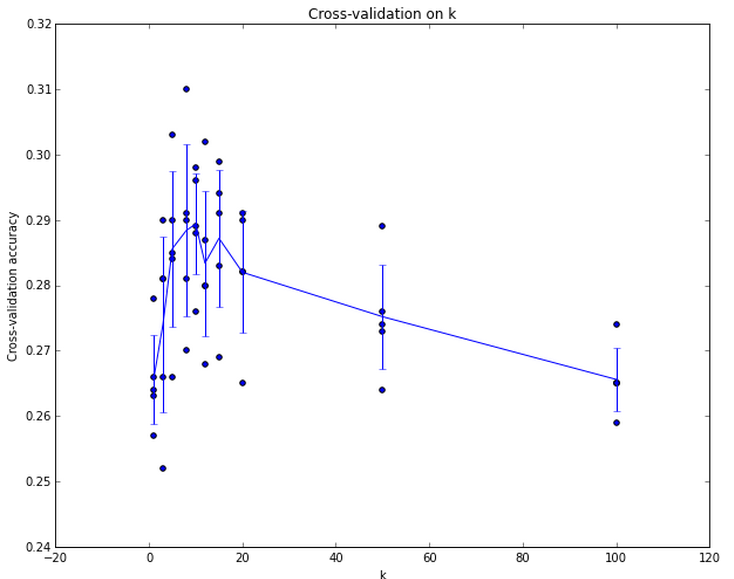
\includegraphics[width=1\textwidth]{knn.png}
  \label{fig2}
  \caption{Example of a 5-fold cross-validation run for the parameter k.}
\end{figure}

\subsubsection{Pros and cons of Nearest Neighbor Classifier}
\paragraph{Pros}
\leavevmode \\
1. It is very simple to implement and understand.
\leavevmode \\
2.  The classifier takes no time to train.
\paragraph{Cons}
\leavevmode \\
1. Accuracy rate is bad. 
\\
2. The classifier must remember all of the training data and store it for future comparisons.
\\
3. Using pixel differences to compare images is inadequate(Figure \ref{fig3})

\begin{figure}[h!]
  \centering
  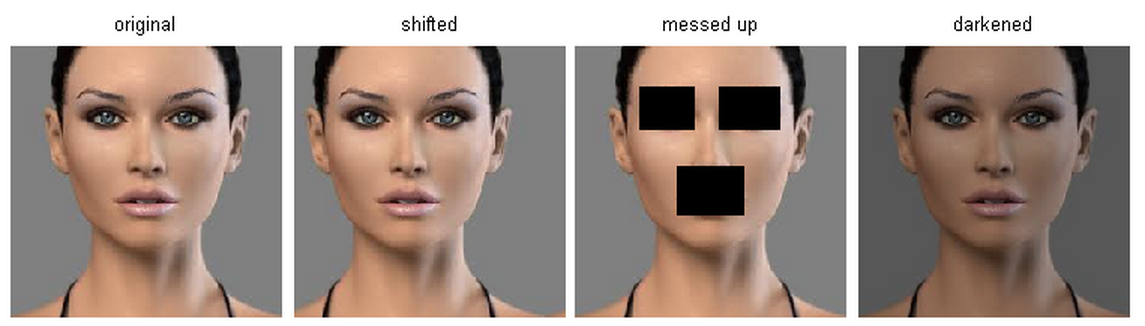
\includegraphics[width=1\textwidth]{consknn.png}
  \caption{Pixel-based distances on high-dimensional data (and images especially) can be very unintuitive. An original image (left) and three other images next to it that are all equally far away from it based on L2 pixel distance. Clearly, the pixel-wise distance does not correspond at all to perceptual or semantic similarity.}
  \label{fig3}
\end{figure}


\section{Linear Classification}
This approach will have two major components: a score function that maps the raw data to class scores, and a loss function that quantifies the agreement between the predicted scores and the ground truth labels. 


\paragraph{Score Function}
\leavevmode \\
For the score function we will use this linear mapping function:
\begin{equation}
 f(x_{i},W,b) = Wx_{i}+b
 \end{equation}
 
In the above equation, we are assuming that the image $x_{i}$ has all of its pixels flattened out to a single column vector of shape $[D*1]$. The matrix $W$ (of size $[K * D]$), and the vector b (of size $[K * 1]$) are the parameters of the function. In CIFAR-10 each image were of size $[32*32*3]$. Here  $x_{i}$ contains all pixels in the i-th image flattened into a single $[3072 * 1]$ column, W is $[10 * 3072]$ and b is $[10 * 1]$, so 3072 numbers come into the function (the raw pixel values) and 10 numbers come out (the class scores). The parameters in W are often called the weights, and b is called the bias vector because it influences the output scores.\hfill \break
An advantage of this approach is that the training data is used to learn the parameters W,b, but once the learning is complete we can discard the entire training set and only keep the learned parameters.
\paragraph{Cost Function}
\leavevmode \\
We will use a loss function called the Multiclass Support Vector Machine (SVM) loss. The SVM loss is set up so that the SVM wants the correct class for each image to a have a score higher than the incorrect classes by some fixed margin $\triangle$. So in each iteration if we achieve lower loss, then it is better. The Multiclass SVM loss for the i-th sample is :

\begin{equation}
 L_{i} =\sum_{i\not=j}max(0,f(x_{i},W)_{j}-f(x_{i},W)_{y_{i}}+\triangle)
 \end{equation}
 
\paragraph{Regularization}
There is an issue with loss function e.g. this set of W is not necessarily unique: there might be many similar W that correctly classify the examples. We can encode some preference for a certain set of weights W over others to remove this ambiguity. We can do so by extending the loss function with a regularization penalty $R(W)$.

\begin{equation}
R(W)=\sum_{k}\sum_{l}W_{k,l}^2 
\end{equation}

We told earlier that Multiclass Support Vector Machine loss is made up of two components: the data loss (which is the average loss $L_{i}$ over all examples) and the regularization loss. So the full Multiclass SVM loss becomes:

\begin{equation}
L= \dfrac{1}{N}\sum_{i}L_{i}+\lambda R(w)
\end{equation}


\section{Softmax Classifier}
In the Softmax classifier, the function mapping is as we used before on linear classifier. But we now interpret these scores as the unnormalized log probabilities for each class. Here we have a cross-entropy loss that has the form:
\begin{equation}
L_{i}=-log(\dfrac{e^{f_{y_{i}})}}{\sum_{j} e^{f_{j}}}
\end{equation}

\section{Optimization : Gradient Descent}
We need to improve our weight vector so that we can get lower loss. We need lower loss because loss function quantifies the agreement between the predicted scores and the ground truth labels. So obtaining lower loss means we are achieving better results. If we do a random search for best direction, then the computational cost will be higher. We can use gradient descent to compute the best direction along which we should change our weight vector. This direction will be related to the gradient of the loss function. This approach roughly corresponds to feeling the slope of the hill below our feet and stepping down the direction that feels steepest. The gradient is just a vector of slopes (more commonly referred to as derivatives) for each dimension in the input space.\hfill \break

By computing Gradient Descent, we are making an update of weight in the negative direction of the gradient since we wish our loss function to decrease, not increase.\hfill \break

Finally with the gradient descent we applied on SVM we get the decreasing loss in Figure 3.3. Also the accuracy was around $37\%$.
\begin{figure}[h!]
  \centering
  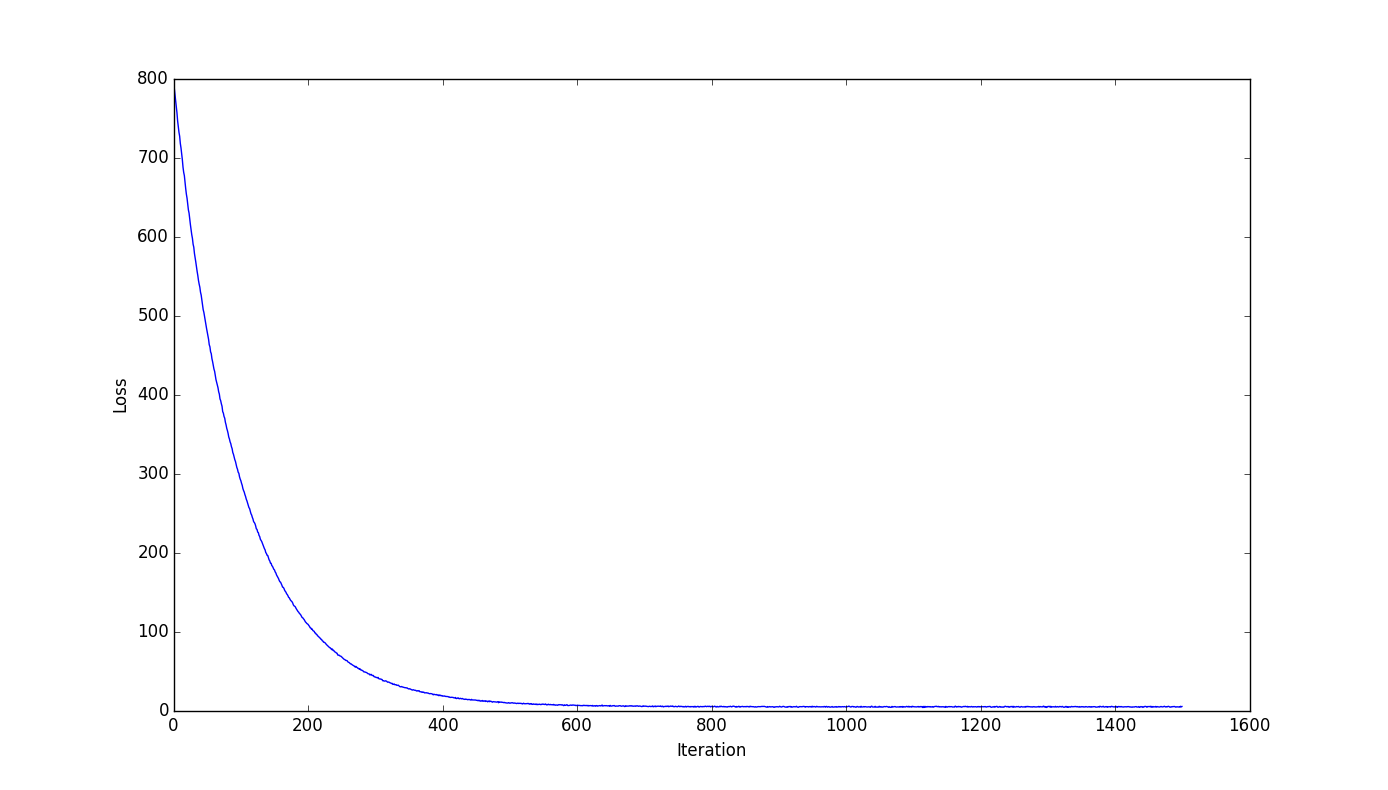
\includegraphics[width=1\textwidth]{svm.png}
  \caption{Decreasing loss as iteration increases}
  \label{fig4}
\end{figure}

\section{Neural Network in Object Detection}
Neural Networks are modeled as collections of neurons that are connected in an acyclic graph. In other words, the outputs of some neurons can become inputs to other neurons. For regular neural networks, the most common layer type is the fully-connected layer in which neurons between two adjacent layers are fully pairwise connected, but neurons within a single layer share no connections. 
\begin{figure}[h!]
  \centering
  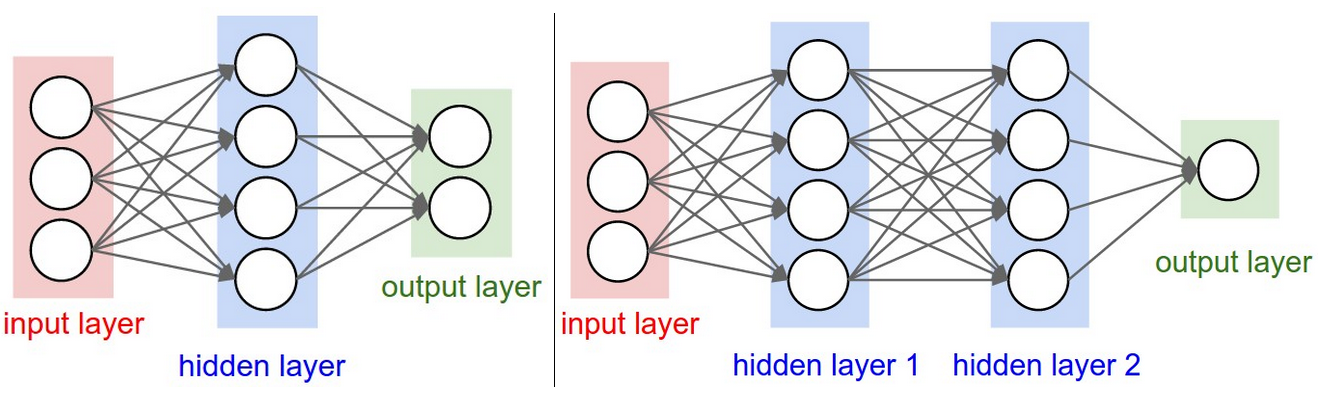
\includegraphics[width=0.7\textwidth]{neural.png}
  \caption{Left: A 2-layer Neural Network (one hidden layer of 4 neurons (or units) and one output layer with 2 neurons), and three inputs. Right: A 3-layer neural network with three inputs.}
  \label{fig5}
\end{figure}
\subsubsection{More Layers Better?}

If we increase the size and number of layers in a Neural Network, the capacity of the network increases. That is, the space of representable functions grows since the neurons can collaborate to express many different functions. In the Figure \ref{fig6} we see that higher hidden neuron means better representational power but it comes with a cost. The problem is overfitting.

\subsubsection{Overfitting}

Overfitting occurs when a model with high capacity fits the noise in the data instead of the underlying relationship. For example, the model with 20 hidden neurons fits all the training data but at the cost of segmenting the space into many disjoint red and green decision regions. A model which has been overfit will generally have poor performance on new data, as it can exaggerate minor fluctuations in the training set.

\begin{figure}[h!]
  \centering
  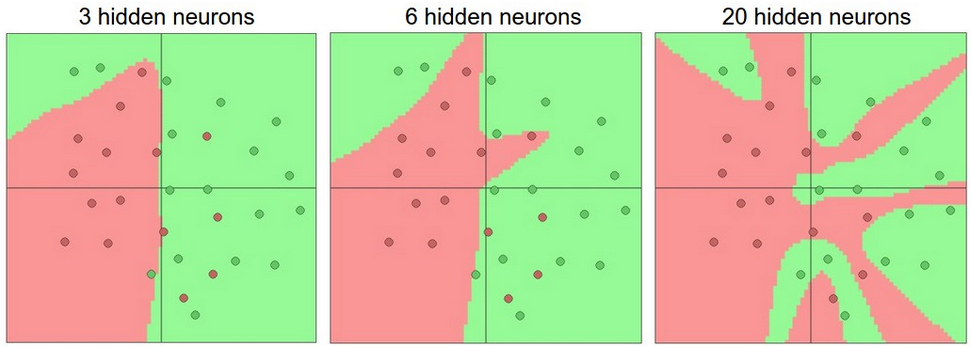
\includegraphics[width=1\textwidth]{neural2.png}
  \caption{Larger Neural Networks can represent more complicated functions. But more layers can also cause overfitting(example with 20 hidden neurons)}
  \label{fig6}
\end{figure}

\begin{figure}[h!]
  \centering
  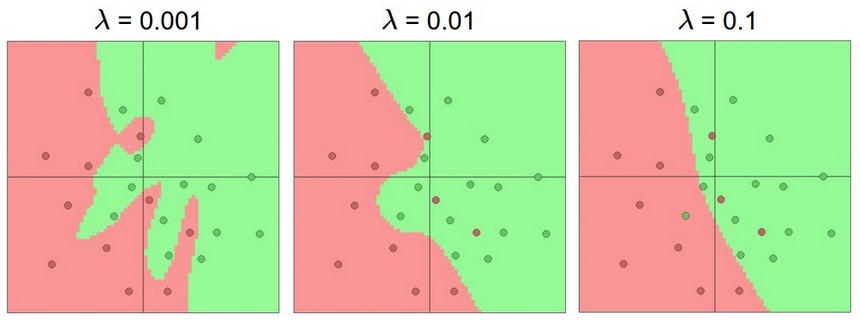
\includegraphics[width=1\textwidth]{neural3.png}
  \caption{The effects of regularization strength}
  \label{fig7}
\end{figure}

\subsubsection{How to control the overfitting?}
Regularization strength is the preferred way to control the overfitting of a neural network.

\begin{figure}[h!]
  \centering
  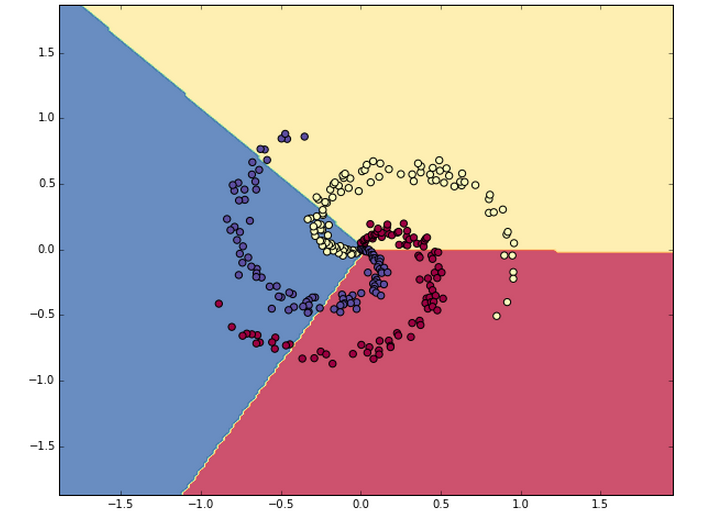
\includegraphics[width=.7\textwidth]{neural4.png}
  \caption{Linear classifier fails to learn the spiral dataset. Accuracy was around $49\%$}
  \label{fig8}
\end{figure}

\begin{figure}[h!]
  \centering
  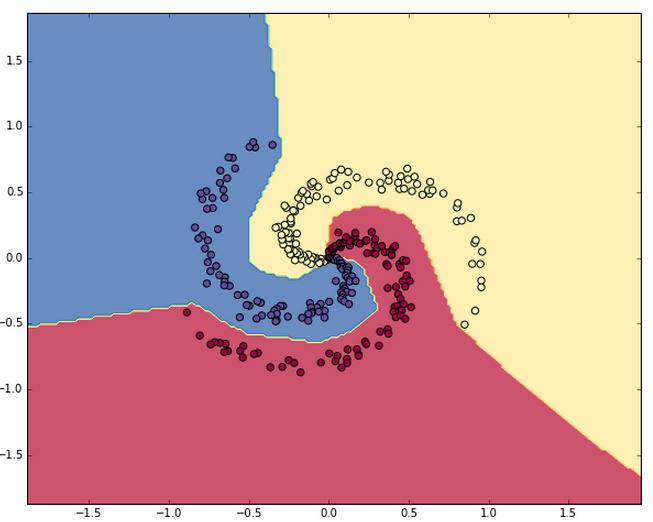
\includegraphics[width=.7\textwidth]{neural5.png}
  \caption{Neural Network classifier is significantly better achieving around $98\%$ accuracy}
  \label{fig9}
\end{figure}


\subsubsection{Linear Classifier vs. Neural Network}
If we implement a 2D dataset and tell any linear classifier to identify, it will fail to identify it correctly. Consider a spiral dataset containing 3 colors:yellow,blue and red. Now if we implement a linear classifier to identify each color in the 2D space we get a result similar to Figure \ref{fig8}.\hfill \break


If we use one additional hidden layer then we can get a lot better result.
\leavevmode
\\
Here we see that adding one additional layer helped us to attain bigger and better functionality.







\chapter{Dataset}
\section{Single Label Dataset}
\subsection{CIFAR-10 Dataset}

The CIFAR-10 dataset is a subset of the 80 million tiny images. They were collected by Alex Krizhevsky, Vinod Nair, and Geoffrey Hinton.\hfill \break 

The CIFAR-10 dataset consists of 60000 32x32 color images in 10 classes, with 6000 images per class. There are 50000 training images and 10000 test images. \hfill \break

The dataset is divided into five training batches and one test batch, each with 10000 images. The test batch contains exactly 1000 randomly-selected images from each class. The training batches contain the remaining images in random order, but some training batches may contain more images from one class than another. Between them, the training batches contain exactly 5000 images from each class. The sample from CIFAR-10 dataset is given in Figure \ref{cifar10}.

\begin{figure}[h!]
  \centering
  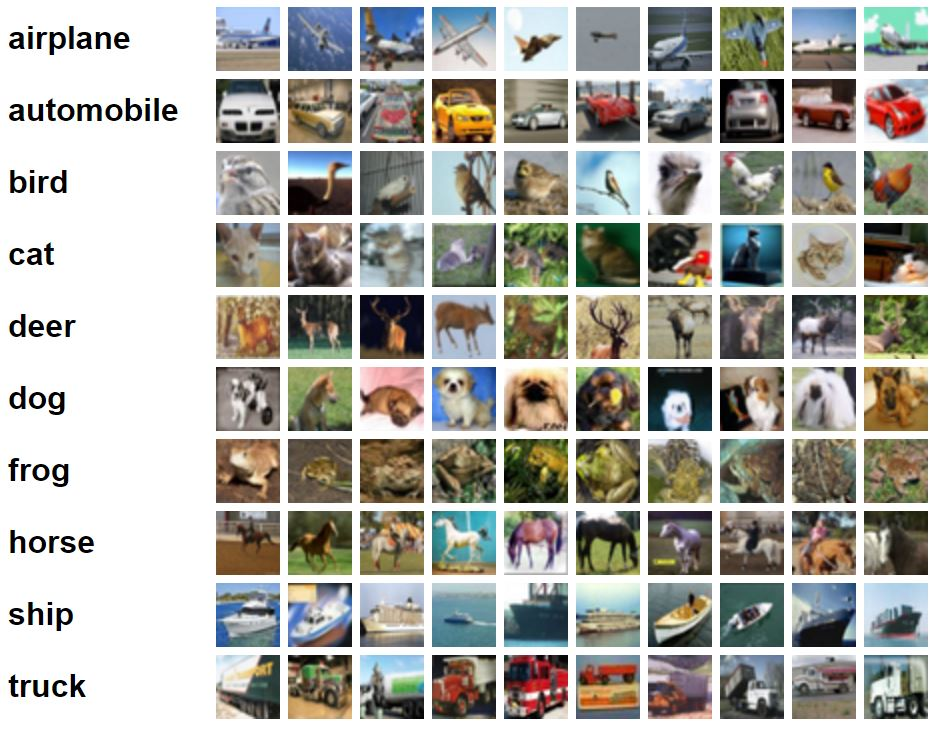
\includegraphics[width=.8\textwidth]{cifar10.JPG}
  \caption{CIFAR-10 Dataset} \label{cifar10}
\end{figure}

\section{Multi Label Dataset}
As we are using single label dataset(CIFAR-10) for our single label Convolutional Neural Network, we have to use images that contain the identical contents from CIFAR-10. So, we picked random 100 images containing the identical contents as CIFAR-10 and tested it with our model. For an example, from Figure \ref{multi} we see that the image contains only a cat and a  dog, which our Single Label Convolutional Network can classify. So, the images we chose only contains subset of airplane, automobile, bird, cat, deer, dog, frog, horse, ship, truck.  

\begin{figure}[h!]
  \centering
  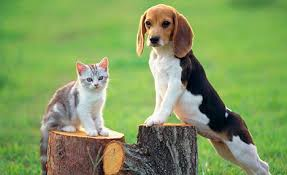
\includegraphics[width=.8\textwidth]{multi.jpg}
  \caption{Multi Label Image} \label{multi}
\end{figure}

\chapter{The Architecture}
\section{The Architecture}\label{sec:SysArchi}

\subsection{Architecture for classifying single label images}
In the figure \ref{singlelabel} is a cropped down version of the Convolutional Neural Network that is used to classify single label images. This has been given to give an idea about the network.

\begin{figure}[h!]
  \centering
  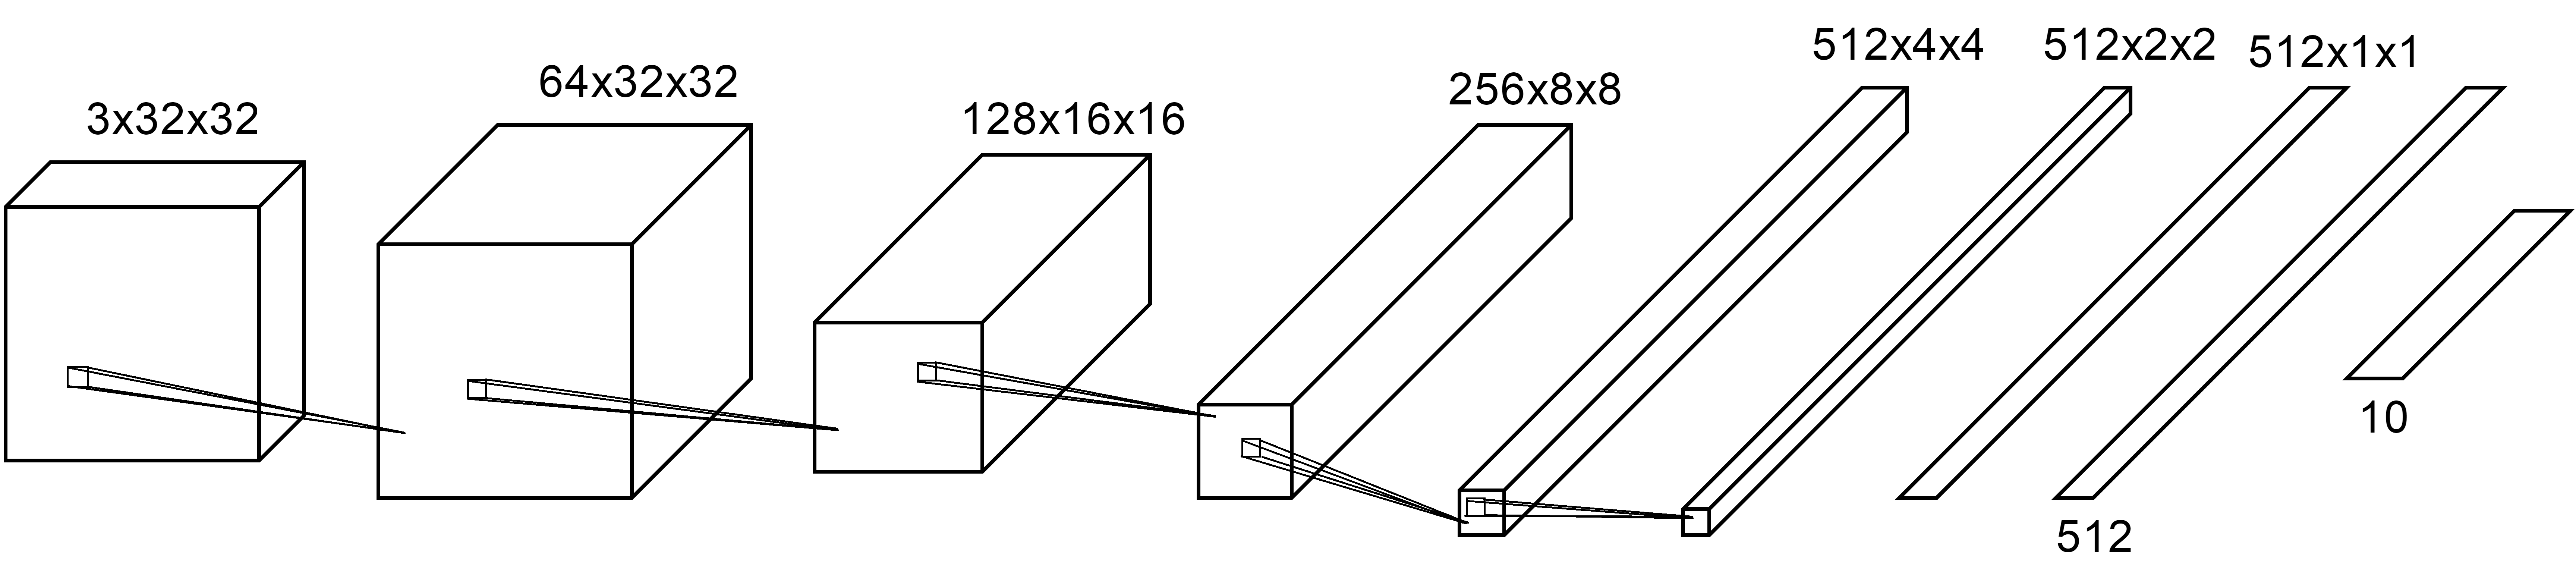
\includegraphics[width=.9\textwidth]{singlelabel.png}
  \caption{Convolutional Neural Network for classifying single label images(Cropped Down)} \label{singlelabel}
\end{figure}

The full network is like the one in the figure. It has 59 layers in sequential manner. The input is the image and output is the label associated with that image.\hfill\break input\(\rightarrow\)1\(\rightarrow\)2\(\rightarrow\)3) \(\rightarrow\) (4) \(\rightarrow\) (5) \(\rightarrow\) (6) \(\rightarrow\) (7) \(\rightarrow\) (8) \(\rightarrow\) (9) \(\rightarrow\) (10) \(\rightarrow\) (11) \(\rightarrow\) (12) \(\rightarrow\) (13) \(\rightarrow\) (14) \(\rightarrow\) (15) \(\rightarrow\) (16) \(\rightarrow\) (17) \(\rightarrow\) (18) \(\rightarrow\) (19) \(\rightarrow\) (20) \(\rightarrow\) (21) \(\rightarrow\) (22) \(\rightarrow\) (23) \(\rightarrow\) (24) \(\rightarrow\) (25) \(\rightarrow\) (26) \(\rightarrow\) (27) \(\rightarrow\) (28) \(\rightarrow\) (29) \(\rightarrow\) (30) \(\rightarrow\) (31) \(\rightarrow\) (32) \(\rightarrow\) (33) \(\rightarrow\) (34) \(\rightarrow\) (35) \(\rightarrow\) (36) \(\rightarrow\) (37) \(\rightarrow\) (38) \(\rightarrow\) (39) \(\rightarrow\) (40) \(\rightarrow\) (41) \(\rightarrow\) (42) \(\rightarrow\) (43) \(\rightarrow\) (44) \(\rightarrow\) (45) \(\rightarrow\) (46) \(\rightarrow\) (47) \(\rightarrow\) (48) \(\rightarrow\) (49) \(\rightarrow\) (50) \(\rightarrow\) (51) \(\rightarrow\) (52) \(\rightarrow\) (53) \(\rightarrow\) (54) \(\rightarrow\) (55) \(\rightarrow\) (56) \(\rightarrow\) (57) \(\rightarrow\) (58) \(\rightarrow\) (59) \(\rightarrow\) output
\hfill\break
A short description about each layer is given below.\hfill\break (1): Spatial Convolution(3 \(\rightarrow\) 64, 3x3, 1,1, 1,1) \hfill\break
  (2): Spatial Batch Normalization \hfill\break
  (3): ReLU \hfill\break
  (4): Dropout(0.3) \hfill\break
  (5): Spatial Convolution(64 \(\rightarrow\) 64, 3x3, 1,1, 1,1) \hfill\break
  (6): Spatial Batch Normalization \hfill\break
  (7): ReLU \hfill\break
  (8): Spatial Max Pooling(2,2,2,2) \hfill\break
  (9): Spatial Convolution(64 \(\rightarrow\) 128, 3x3, 1,1, 1,1) \hfill\break
  (10): Spatial Batch Normalization \hfill\break
  (11): ReLU \hfill\break
  (12): Dropout(0.4) \hfill\break
  (13): Spatial Convolution(128 \(\rightarrow\) 128, 3x3, 1,1, 1,1) \hfill\break
  (14): Spatial Batch Normalization \hfill\break
  (15): ReLU \hfill\break
  (16): Spatial Max Pooling(2,2,2,2) \hfill\break
  (17): Spatial Convolution(128 \(\rightarrow\) 256, 3x3, 1,1, 1,1) \hfill\break
  (18): Spatial Batch Normalization \hfill\break
  (19): ReLU \hfill\break
  (20): Dropout(0.4) \hfill\break
  (21): Spatial Convolution(256 \(\rightarrow\) 256, 3x3, 1,1, 1,1) \hfill\break
  (22): Spatial Batch Normalization \hfill\break
  (23): ReLU \hfill\break
  (24): Dropout(0.4) \hfill\break
  (25): Spatial Convolution(256 \(\rightarrow\) 256, 3x3, 1,1, 1,1) \hfill\break
  (26): Spatial Batch Normalization \hfill\break
  (27): ReLU \hfill\break
  (28): Spatial Max Pooling(2,2,2,2) \hfill\break
  (29): Spatial Convolution(256 \(\rightarrow\) 512, 3x3, 1,1, 1,1) \hfill\break
  (30): Spatial Batch Normalization \hfill\break
  (31): ReLU \hfill\break
  (32): Dropout(0.4) \hfill\break
  (33): Spatial Convolution(512 \(\rightarrow\) 512, 3x3, 1,1, 1,1) \hfill\break
  (34): Spatial Batch Normalization \hfill\break
  (35): ReLU \hfill\break
  (36): Dropout(0.4) \hfill\break
  (37): Spatial Convolution(512 \(\rightarrow\) 512, 3x3, 1,1, 1,1) \hfill\break
  (38): Spatial Batch Normalization \hfill\break
  (39): ReLU \hfill\break
  (40): Spatial Max Pooling(2,2,2,2) \hfill\break
  (41): Spatial Convolution(512 \(\rightarrow\) 512, 3x3, 1,1, 1,1) \hfill\break
  (42): Spatial Batch Normalization \hfill\break
  (43): ReLU \hfill\break
  (44): Dropout(0.4) \hfill\break
  (45): Spatial Convolution(512 \(\rightarrow\) 512, 3x3, 1,1, 1,1) \hfill\break
  (46): Spatial Batch Normalization \hfill\break
  (47): ReLU \hfill\break
  (48): Dropout(0.4) \hfill\break
  (49): Spatial Convolution(512 \(\rightarrow\) 512, 3x3, 1,1, 1,1) \hfill\break
  (50): Spatial Batch Normalization \hfill\break
  (51): ReLU \hfill\break
  (52): Spatial Max Pooling(2,2,2,2) \hfill\break
  (53): View \hfill\break
  (54): Dropout(0.5) \hfill\break
  (55): Linear(512 \(\rightarrow\) 512) \hfill\break
  (56): Batch Normalization \hfill\break
  (57): ReLU \hfill\break
  (58): Dropout(0.5) \hfill\break
  (59): Linear(512 \(\rightarrow\) 10) \hfill\break
  
  
  \paragraph{Spatial Convolution:}
  
  Applies a 2D convolution over an input image composed of several input planes. For an example, Spatial Convolution(3 \(\rightarrow\) 64, 3x3, 1,1, 1,1) means that number of input channel is 3, and the number of output channel is 64. The kernel size is 3x3 and as there are 64 output channels, there will be 64 kernels, each having dimension 3x3. The step of the convolution is 1 step for height and width. The padding is 1 for height and width. Let's visualize this. In the figure \ref{spatialconv} the input neurons are the ones representing each pixel of an image, the kernel size or the filter size is 5x5. This filter would iterate over every single pixel and for each pixel look at the 5x5 neighborhood and produce corresponding images. As the number of output channel is 64, this will be done 64 times.
  
  \begin{figure}[h!]
  \centering
  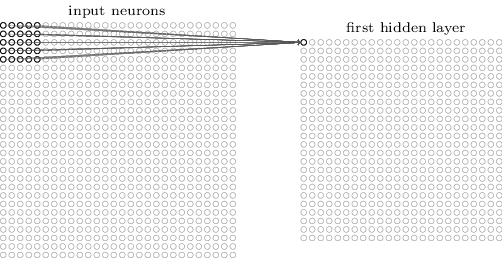
\includegraphics[width=.9\textwidth]{spatialconv.png}
  \caption{Spatial Convolution with kernel size 5x5} \label{spatialconv}
\end{figure}

\paragraph{Spatial Batch Normalization:}

Implements Batch Normalization as described in the paper \cite{26}. The operation implemented is:

 $$y=\frac{x - mean(x)}{standard-deviation(x)} * gamma + beta$$
 
 where the mean and standard-deviation are calculated per feature-map over the mini-batches and pixels and where gamma and beta are learnable parameter vectors of size N (where N = number of feature maps).
 
 
 \paragraph{ReLU:}
 It is the activation function defined as: $$f(x) = max(0,x)$$.
 
 
 \paragraph{Spatial Max Pooling:}
 Applies 2D max-pooling operation. For example, Spatial Max Pooling(2,2,2,2) means that the max pooling will be done with filter 2x2 with step 2 in height and step 2 in width direction. Max pooling means that we will select the maximum value from 2x2 filter or the input area.
 
 
 \paragraph{Dropout:}
 Dropout is used to prevent the neural network from overfitting. Dropout is implemented by only keeping a neuron active with some probability p (a hyperparameter), or setting it to zero otherwise. The input neuron is scaled by $1/p$ if it is not deactivated.
 
 \paragraph{Linear:}
 Applies a linear transformation to the incoming data ($y = mx + c$). For example, Linear(512 \(\rightarrow\) 10) means that there are 512 input channels and these 512 channels are converted to 10 channels. So, the weight matrix will be 10x512. 
 
 
 \paragraph{Loss Function:}
 Cross-entropy loss function has been used which has the form:
 
 
$$ L_{i} = -\log{(\frac{e^{f_y}}{\sum_j{e^{f_j}}})}$$

\subsection{Normalization on CIFAR-10}

Normalization is required so that all the inputs are at a comparable range. This can be done to force the input values to a certain range. The images were converted from RGB channel to YUV channel. Then U and V channels were normalized globally with mean and standard deviation. The Y channel was normalized locally.

\section{Object Recognition}
There are many approaches for segmenting an image having multiple objects into many segmented images. Our target is to take any approach and pass it to our trained CNN model. We found out two established approaches and tried on that.

\subsection{Measuring the objectness of image windows}
B. Alexe et al. \cite{15} presented a generic objectness measure, quantifying how likely it is for an image window to contain an object of any
class. They explicitly trained it to distinguish objects with a well-defined boundary in space, such as cows and telephones, from amorphous
background elements, such as grass and road. The measure combines in a Bayesian framework several image cues measuring
characteristics of objects, such as appearing different from their surroundings and having a closed boundary. These include an
innovative cue to measure the closed boundary characteristic. Finally, they presented two applications of objectness. In the first, they sample a small number windows according to their
objectness probability and gave an algorithm to employ them as location priors for modern class-specific object detectors. As they showed

\begin{figure}[ht] 
  \begin{subfigure}[b]{0.5\linewidth}
    \centering
    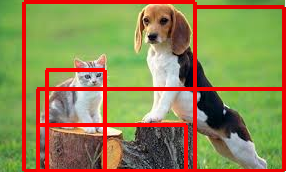
\includegraphics[width=0.9\linewidth]{obj1}
    \caption{} 
    \label{obj1} 
    \vspace{4ex}
  \end{subfigure}%%
  \begin{subfigure}[b]{0.5\linewidth}
    \centering
    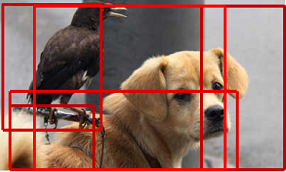
\includegraphics[width=0.9\linewidth]{obj2}
    \caption{} 
    \label{obj2} 
    \vspace{4ex}
  \end{subfigure}%%
  \caption{}
  \label{objectnessfig} 
\end{figure}

experimentally, this greatly reduces the number of windows evaluated by the expensive class-specific model. In the second application,
they used objectness as a complementary score in addition to the class-specific model, which leads to fewer false positives. As shown in
several recent papers, objectness can act as a valuable focus of attention mechanism in many other applications operating on image
windows, including weakly supervised learning of object categories, unsupervised pixelwise segmentation, and object tracking in video.
Computing objectness is very efficient and takes only about 4 sec. per image. This technique finds out some image windows like Figure \ref{objectnessfig}. \hfill \break

\begin{algorithm}[H]
\SetAlgoLined
\begin{description}\itemsep1pt \parskip0pt \parsep0pt \vspace{.5cm}
  \item[Input:] \(F, D, C\) 
  \item[Ouput:] \(Det\)
  \item[Step 1:] \( \l = \left \{ w_{1},...,w_{F} \right \}, w_{i}\rightarrow D, \forall_{i} \)
  \item[Step 2:] \( \l_{s} = \left \{ \left ( w_{1},sw_{1} \right ),...,\left ( w_{F},sw_{F} \right )  \right \}, sw_{i}= c\left ( w_{i} \right ), \forall_{i} \) 
  \item[Step 3:] \( \rho _{s} = NMS\left ( \l_{s} \right )=\left \{ \left ( w_{n1},sw_{n1} \right ),...,\left ( w_{np},sw_{np} \right )  \right \}\)
  \item[Step 4:] \(\L=\left \{ w_{n1}^{lm},..., w_{np}^{lm} \right \}, w_{nj}^{lm} = max \left ( s_{w} \right )\)
  \item[Step 5:] \(Det = NMS\left ( \L \right )\)
\end{description}
\caption{Using objectness for class-specific detectors.}
\end{algorithm}

\hfill \break
The general scheme for using their objectness measure as
a location prior for object detectors is algorithm 1. The
algorithm inputs the class-specific confidence function \(c\) which
the detector employs to score a window.
They build an initial set \(I\) of \(F = 1000\) windows multinomially sampled from the distribution \(D\) of windows scored by
their objectness measure (Multi-scale Saliency)\(MS\) +(Color Contrast)\(CC\) + (Superpixels Straddling)\(SS\) (step 1). They use \(c\) to
score each window in \(I\) (step 2). We then run the non-maxima
suppression. This results in a set \(\rho_{s}\) of promising
windows (step 3). For every window \(w_{p} \epsilon \rho_{s}\), they iteratively
move to the local maximum of \(c\) in its neighborhood \(V_{w
p}\),
resulting in window \(w_{p}^{lm}\) (step 4). Finally, they run \(NMS\) on the
local maxima windows \(\L\) and obtain detections \(Det\) (step 5).
In order to use this algorithm one has to specify a window
scoring function \(c\), which is specific to a particular detector
and object class, and a window neighborhood.



\subsection{Selective Search for Object Recognition}

%\begin{algorithm}[H]
%\SetAlgoLined
%\KwData{(color) image}
%\KwResult{Set of object location hypotheses \(L\) }\break
% Obtain initial regions \(R = \left \{ r_{1},..., r_{n} \right \}\) using [13]\break
% Initialize similarity set \(S = \varnothing\)
% \foreach{abc}
% \While{While condition}{
%  instructions\;
%  \eIf{condition}{
%   instructions1\;
%   instructions2\;
%   }{
%   instructions3\;
%  }
% }
% \caption{How to write algorithms}
%\end{algorithm}

J.R.R. Uijlings et al. \cite{16} took a hierarchical grouping algorithm to form the basis of their
selective search. Bottom-up grouping is a popular approach to segmentation \cite{24} \cite{25}, hence they adapted it for selective search. Because
the process of grouping itself is hierarchical, they can naturally generate locations at all scales by continuing the grouping process until
the whole image becomes a single region. This satisfies the condition of capturing all scales.
As regions can yield richer information than pixels, they wanted to
use region-based features whenever possible. To get a set of small
starting regions which ideally do not span multiple objects, they used the fast method of Felzenszwalb and Huttenlocher \cite{25}, which
found well-suited for such purpose.
Their grouping procedure now works as follows. They first used \cite{25}
to create initial regions. Then they used a greedy algorithm to iteratively group regions together: First the similarities between all
neighbouring regions are calculated. The two most similar regions
are grouped together, and new similarities are calculated between
the resulting region and its neighbours. The process of grouping
the most similar regions is repeated until the whole image becomes
a single region.


\subsection{Architecture For Classifying Multi-Label Images}

Our Final architecture for detecting multi-label images consists of (1) image segmentation and (2) convolutional neural network for detecting segmented images. The image segmentation techniques, objectness measures and selective search and the architecture for single label image detection has been described before. In the Figure \ref{finalarch} there is an overview of the architecture. \hfill \break

\begin{figure}[h!]
  \centering
  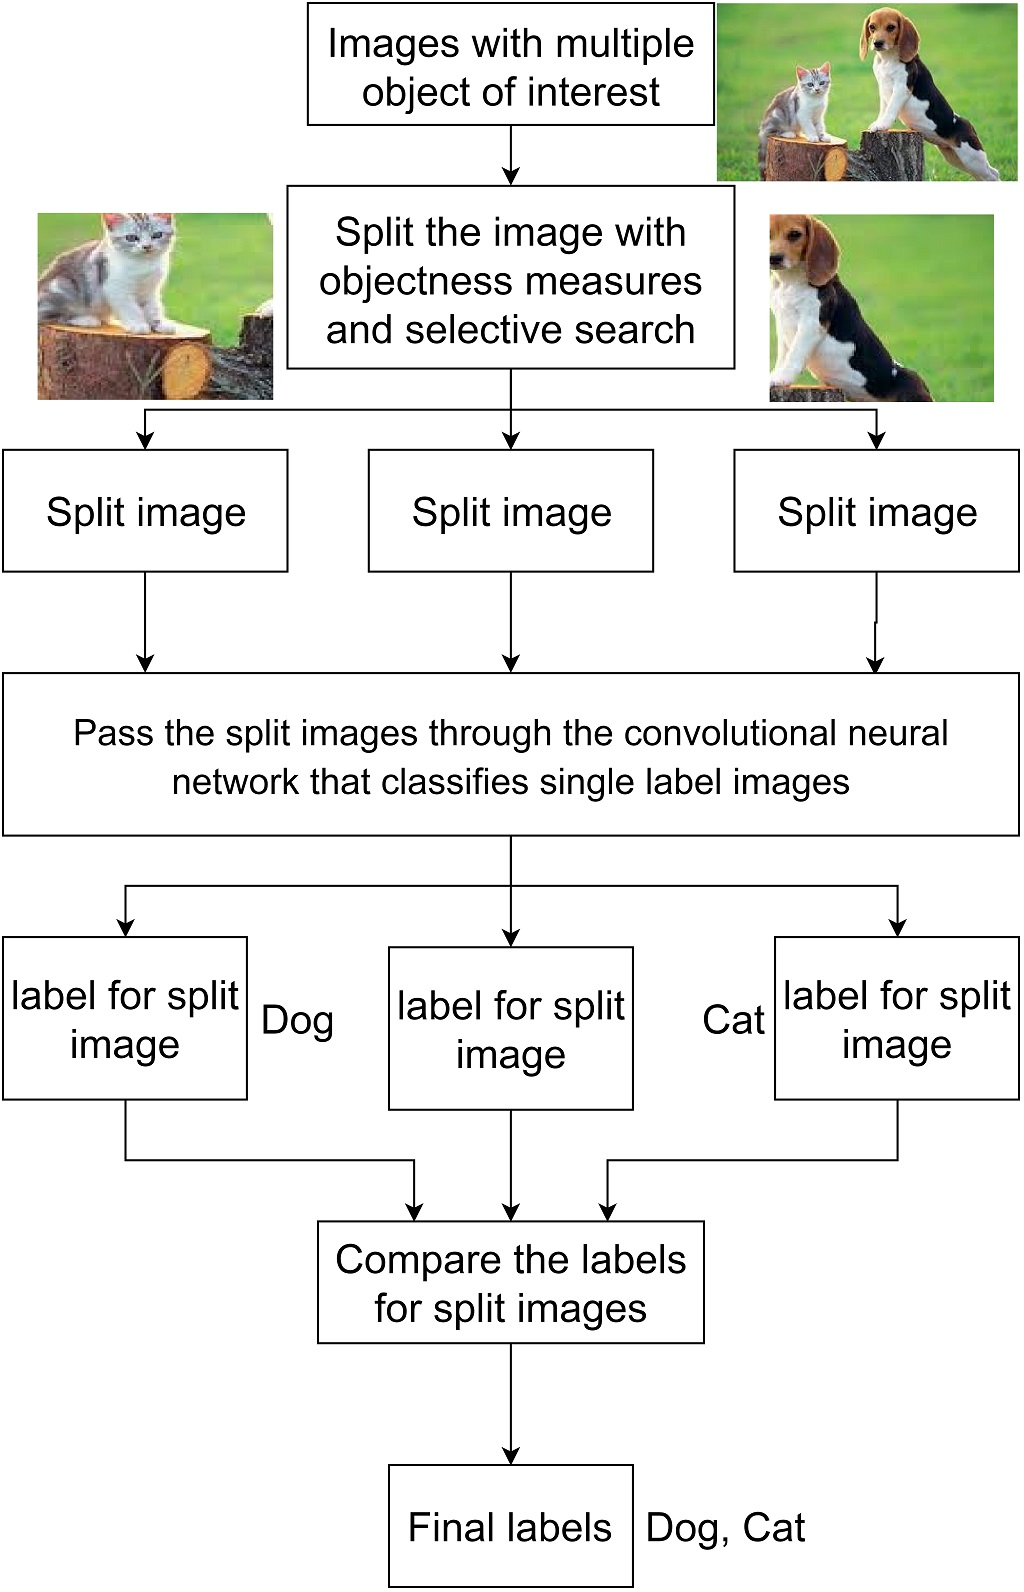
\includegraphics[width=0.9\textwidth]{finalarch.jpg}
  \caption{Architecture of Convolutional neural network}\label{finalarch}
\end{figure}

At first we split the image with objectness measures and selective search. Then we get multiple split images. Note that there will be many split images. In the figure only a few are shown. Then we pass the split images through the convolutional neural network that classifies the label associated with that image. As there are many split images, there may be some labels that will be wrongly classified. We inspect these labels and their associative scores and finally conclude which of the labels are likely to be associated with the images. We performed several techniques for inspecting the images. These are discussed in the experimental result section.



%\chapter{Proposed Algorithm}
%\section{The ADC-QSIN algorithm for scheduling multi-item queries using network coding} 

\chapter{Experimental Result}
\section{Experimental Results}

\subsection{Experimental Result for CIFAR-10}

In the fig \ref{cifar10conf} there is the result for the testing images of CIFAR-10 dataset. Here, each row represents the testing label, each column represents the label produced by the network. For example the cell (1,1) represents that the testing label is airplane and the classified label is airplane, the cell (1,2) represents that the testing label is airplane and the classified label is automobile. So, each cell (i,i) where $[i = 1..10]$ represents the correctly classified labels. Each row consists of 1000 image labels. So the accuracy will be cell$(i,i)/1000$.

\begin{figure}[h!]
  \centering
  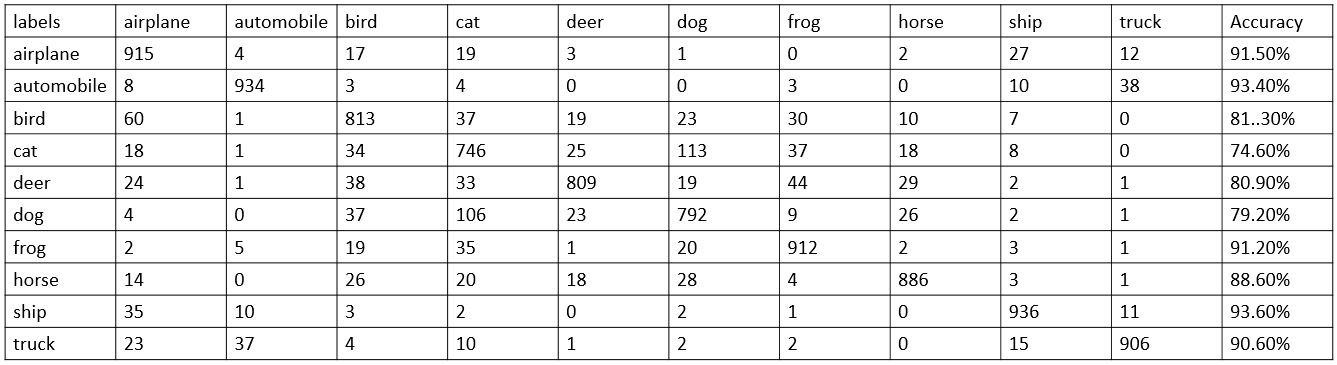
\includegraphics[width=0.9\textwidth]{cifar10.PNG}
  \caption{CIFAR-10 Confusion Matrix}\label{cifar10conf}
\end{figure}





\subsection{Experimental Result for Multi-Label Image Classification}
To give an overview of the process of inspecting the result of the segmented images, we will need the help of Table from Figure \ref{score}. The table is for a single multi-label image. Each $image_{i}$ represents the segmented image from the multi-label image. Each row represents the class scores given by the network. 

\paragraph{Selecting Top-1 Score:}
In this approach we select the top 1 score and its associating label from each segmented image $image_{i}$. Then we increase the frequency of labels for each top 1 score. After that we select the top 4 scoring labels. For example, in the Figure \ref{score} the top 1 label for $image_{1}$ would be cat. So we increase the frequency of cat by 1. Similarly for $image_{2}$ again the score for label cat is highest. So frequency of cat will be increased by 1.

\begin{figure}[h!]
  \centering
  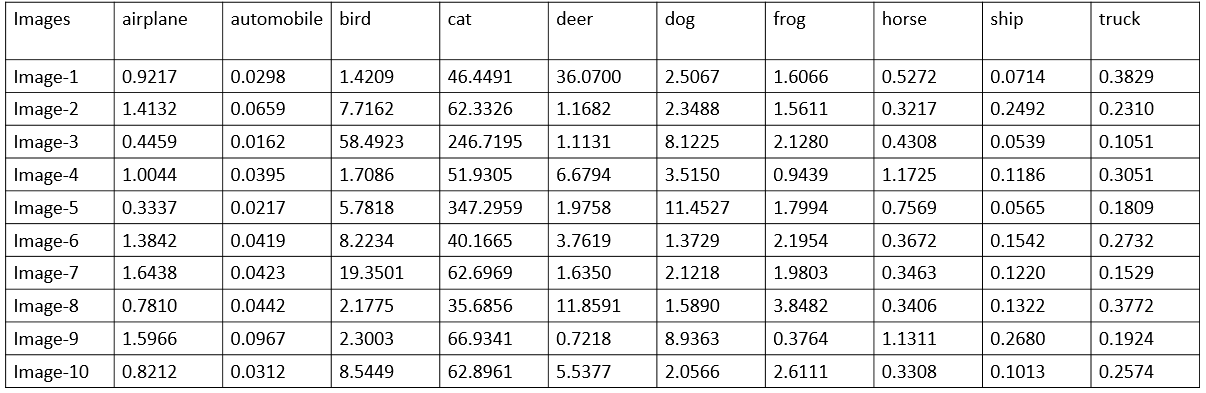
\includegraphics[width=0.9\textwidth]{newresult.PNG}
  \caption{Scores for the sample image}\label{score}
\end{figure}

\paragraph{Selecting Top-2 Score:}
In this approach we select the top 2 scores and its associating label from each segmented image $image_{i}$. Then we increase the frequency of labels for each top 2 scores. After that we select the top 4 scoring labels.  For example, in the Figure \ref{score} the top 2 labels for $image_{1}$ would be cat and deer. So the frequency of cat and deer will be increased by 1.

\begin{figure}[h!]
  \centering
  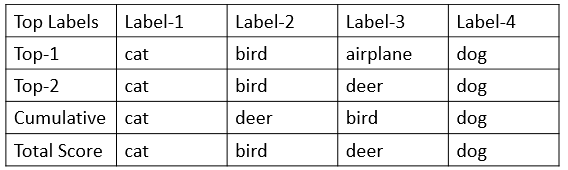
\includegraphics[width=0.9\textwidth]{result_objectness.PNG}
  \caption{Result for the sample image for Objectness Measures}\label{resobj}
\end{figure}

\paragraph{Selecting Total Score:}
In this approach we just add all scores of each $label_{i}$ for each segmented image $image_{i}$. Then we select the top 4 scoring labels. For example, every class score for every label will be added. So, the score for cat label will be the total score in the column cat. Similarly the score for bird will be the total score in the column bird.

\begin{figure}[h!]
  \centering
  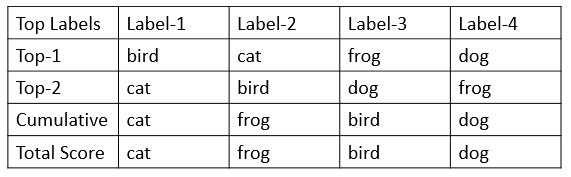
\includegraphics[width=0.9\textwidth]{result_selective.PNG}
  \caption{Result for the sample image for Selective Search}\label{ressel}
\end{figure}



\paragraph{Selecting Cumulative Percentage:}
Each $label_{i}$ of segmented image $image_{i}$ has the percentage $score_{i} / \sum_{i}{score_{i}}$. We select the top percentage from each segmented image $image_{i}$. We add these percentages for each associated labels and select the top 4 scoring labels. For example for $image_{1}$ the percentage of cat will be $score_{cat} / \sum_{i}{score_{i}}$.\hfill \break

The results for these four approaches for the sample image from Figure \ref{sample_multi_label} is given at Figure \ref{resobj} and Figure \ref{ressel} \hfill \break


These approaches were repeated in our selected multi label images. The results for Objectness Measure is given in Figure \ref{finobj} and for Selective Search in Figure  \ref{finsel}

\begin{figure}[h!]
  \centering
  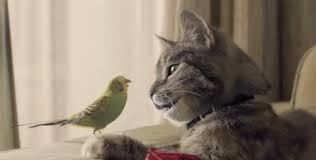
\includegraphics[width=0.5\textwidth]{sample_multi_label.PNG}
  \caption{Sample Multi-Label Image}\label{sample_multi_label}
\end{figure}


\begin{figure}[h!]
  \centering
  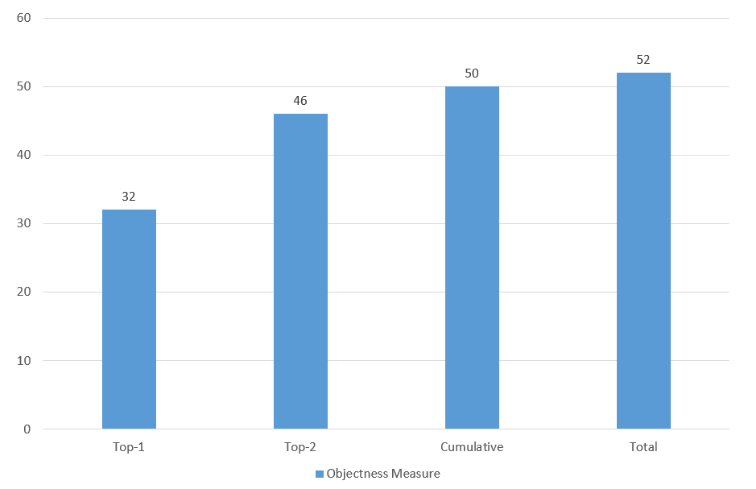
\includegraphics[width=0.5\textwidth]{Capture3.PNG}
  \caption{Result for multi-label images for Objectness Measures}\label{finobj}
\end{figure}


\begin{figure}[h!]
  \centering
  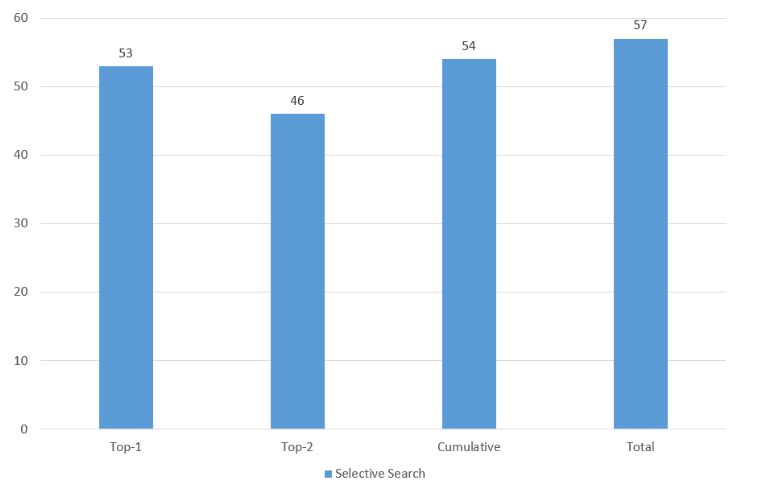
\includegraphics[width=0.5\textwidth]{Capture4.PNG}
  \caption {Result for multi-label images for Selective Search}\label{finsel}
\end{figure}



\chapter{Tools and Recommendations for Future Works}
\section{Used Tools}
\subsubsection{Torch}
Torch is a scientific computing framework with wide support for machine learning algorithms. It is easy to use and efficient. At the heart of Torch are the popular neural network and optimization libraries which are simple to use, while having maximum flexibility in implementing complex neural network topologies.\hfill \break 

Our Convolutional Neural Network runs on top of Torch.

\subsubsection{Waffle}
Waffle is a fast, asynchronous, express-inspired web framework for Torch built on top of ASyNC. \hfill \break

We used this to build a server that classifies the single and multi-label images.

\section{Future Works}
The strength of our multi-label image classification architecture depends on single-label convolutional neural network classifier and the method for segmenting images.\hfill \break

So, be refining out convolutional neural network to include more labels by training CIFAR-100 and using better methods to segment the image, we can improve the performance of the network.

\chapter{Conclusion}
We have presented an easy and simple approach to classify multi-label images using a trained single-label image classifier with objectness measure and selective search of an image. It gave us the result in quick time. Our training time for single-label network is fast. Segmenting the images is also fast. Our technique is a stepping stone to this approach. It is giving a good threshold result. In the future, this model can be enhanced and cope with larger dataset. So it will be interesting to see how advancement is made in this approach.

%\appendix
%\chapter{Appendix}
%\input{chapters/appendix}

\begin{thebibliography}{150}

    % Set Reference ID carefully, do not use replication
    \bibitem {1} L. Fei-Fei, R. Fergus, and P. Perona. Learning generative visual
models from few training examples: An incremental bayesian
approach tested on 101 object categories. Computer Vision and
Image Understanding, 106(1):59–70, 2007.

\bibitem {2} J. Deng, W. Dong, R. Socher, L.-J. Li, K. Li, and L. FeiFei. Imagenet: A large-scale hierarchical image database. In
Computer Vision and Pattern Recognition, pages 248–255, 2009.

\bibitem {3} D. G. Lowe. Distinctive image features from scale-invariant
keypoints. International Journal of Computer Vision, 60(2):91–
110, 2004.

\bibitem {4} S. Lazebnik, C. Schmid, and J. Ponce. Beyond bags of features:
Spatial pyramid matching for recognizing natural scene categories. In Computer Vision and Pattern Recognition, volume 2,
pages 2169–2178, 2006.

\bibitem {5} J. Wang, J. Yang, K. Yu, F. Lv, T. Huang, and Y. Gong. Localityconstrained linear coding for image classification. In Computer
Vision and Pattern Recognition, pages 3360–3367, 2010.

\bibitem {6} C.-C. Chang and C.-J. Lin. Libsvm: a library for support
vector machines. ACM Trans. Intelligent Systems and Technology,
2(3):27, 2011.

\bibitem {7}  L. Breiman. Random forests. Machine learning, 45(1):5–32, 2001.

\bibitem {8} Y. LeCun, B. Boser, J. Denker, D. Henderson, R. Howard,
W. Hubbard, and L. Jackel. Handwritten digit recognition with
a back-propagation network. In Neural Information Processing
Systems, 1990.

\bibitem {9} K. Jarrett, K. Kavukcuoglu, M. Ranzato, and Y. LeCun. What
is the best multi-stage architecture for object recognition? In
International Conference on Computer Vision, pages 2146–2153,
2009.

\bibitem {10} A. Krizhevsky, I. Sutskever, and G. Hinton. Imagenet classification with deep convolutional neural networks. In Neural
Information Processing Systems, pages 1106–1114, 2012.

\bibitem {11} W. Ouyang and X. Wang. Joint deep learning for pedestrian
detection. In International Conference on Computer Vision, pages
2056–2063, 2013.

\bibitem {12} F. Perronnin, J. Sanchez, and T. Mensink. Improving the ´
fisher kernel for large-scale image classification. In European
Conference on Computer Vision, pages 143–156, 2010.

\bibitem {13} Q. Chen, Z. Song, Y. Hua, Z. Huang, and S. Yan. Hierarchical
matching with side information for image classification. In
Computer Vision and Pattern Recognition, pages 3426–3433, 2012.

\bibitem {14} J. Dong, W. Xia, Q. Chen, J. Feng, Z. Huang, and S. Yan.
Subcategory-aware object classification. In Computer Vision and
Pattern Recognition, pages 827–834, 2013.

\bibitem {15} Alexe, B., Deselares, T. and Ferrari.
 Measuring the objectness of image windows. V. PAMI 2012.

\bibitem {16} R. R. Uijlings, Koen E. A. van de Sande, Theo Gevers, Arnold W. M. Smeulders. 
Selective Search for Object Recognition, Jasper  International Journal of Computer Vision, Volume 104 (2), page 154-171, 2013.

\bibitem {17} Dataset of CIFAR-10 https://www.cs.toronto.edu/~kriz/cifar.html.

\bibitem {18} H. Harzallah, F. Jurie, and C. Schmid. Combining efficient
object localization and image classification. In Computer Vision
and Pattern Recognition, pages 237–244, 2009.

\bibitem {19} Y. Gong, Y. Jia, T. K. leung, A. Toshev, and S. Ioffe. deep
convolutional ranking for multi label image annotation. In
International Conference on Learning Representations, 2014.

\bibitem {20} N. Dalal and B. Triggs. Histograms of oriented gradients for
human detection. In Computer Vision and Pattern Recognition,
volume 1, pages 886–893, 2005.

\bibitem {21} T. Ojala, M. Pietikainen, and D. Harwood. A comparative 
study of texture measures with classification based on featured
distributions. Pattern recognition, 29(1):51–59, 1996.

\bibitem {22} N. M. Nasrabadi and R. A. King. Image coding using vector quantization: A review. IEEE Trans. Communications, 36(8):957–
971, 1988.

\bibitem {23} P. Hedelin and J. Skoglund. Vector quantization based on
gaussian mixture models. IEEE Trans. Speech and Audio Processing, 8(4):385–401, 2000.

\bibitem{24} D. Comaniciu and P. Meer. Mean shift: a robust approach
toward feature space analysis. TPAMI, 24:603–619, 2002.

\bibitem{25} P. F. Felzenszwalb and D. P. Huttenlocher. Efficient GraphBased Image Segmentation. IJCV, 59:167–181, 2004. 

\bibitem{26} Sergey Ioffe, Christian Szegedy.
 Batch Normalization: Accelerating Deep Network Training by Reducing
Internal Covariate Shift.

\end{thebibliography}


\end{document}
